\label{sec:guidelines_content}
The thesis work must be printed, hole punched, bound with twine, sealed with a sticker/signature, and placed in an official book (Fig.~\ref{fig:binding}). The binding book comes in a few colors such as green, blue, and red and can be bought at Bookvoed. Just make sure to buy the correct version, as there are other options for other degrees. (e.g. for bachelor's degree work)

After passing the formatting check and receiving signatures, the thesis can be bound up. Tip: Get it checked digitally, rather than printing in advance. When you are ready to bind, visit the office and Elena will provide twine and a signature label. This goes through the holes of the paper so no pages can be changed. Finally, it can be put into the binding book and submitted to Elena.

%Figure: Binding Book
\begin{figure}[H]
    \centering
    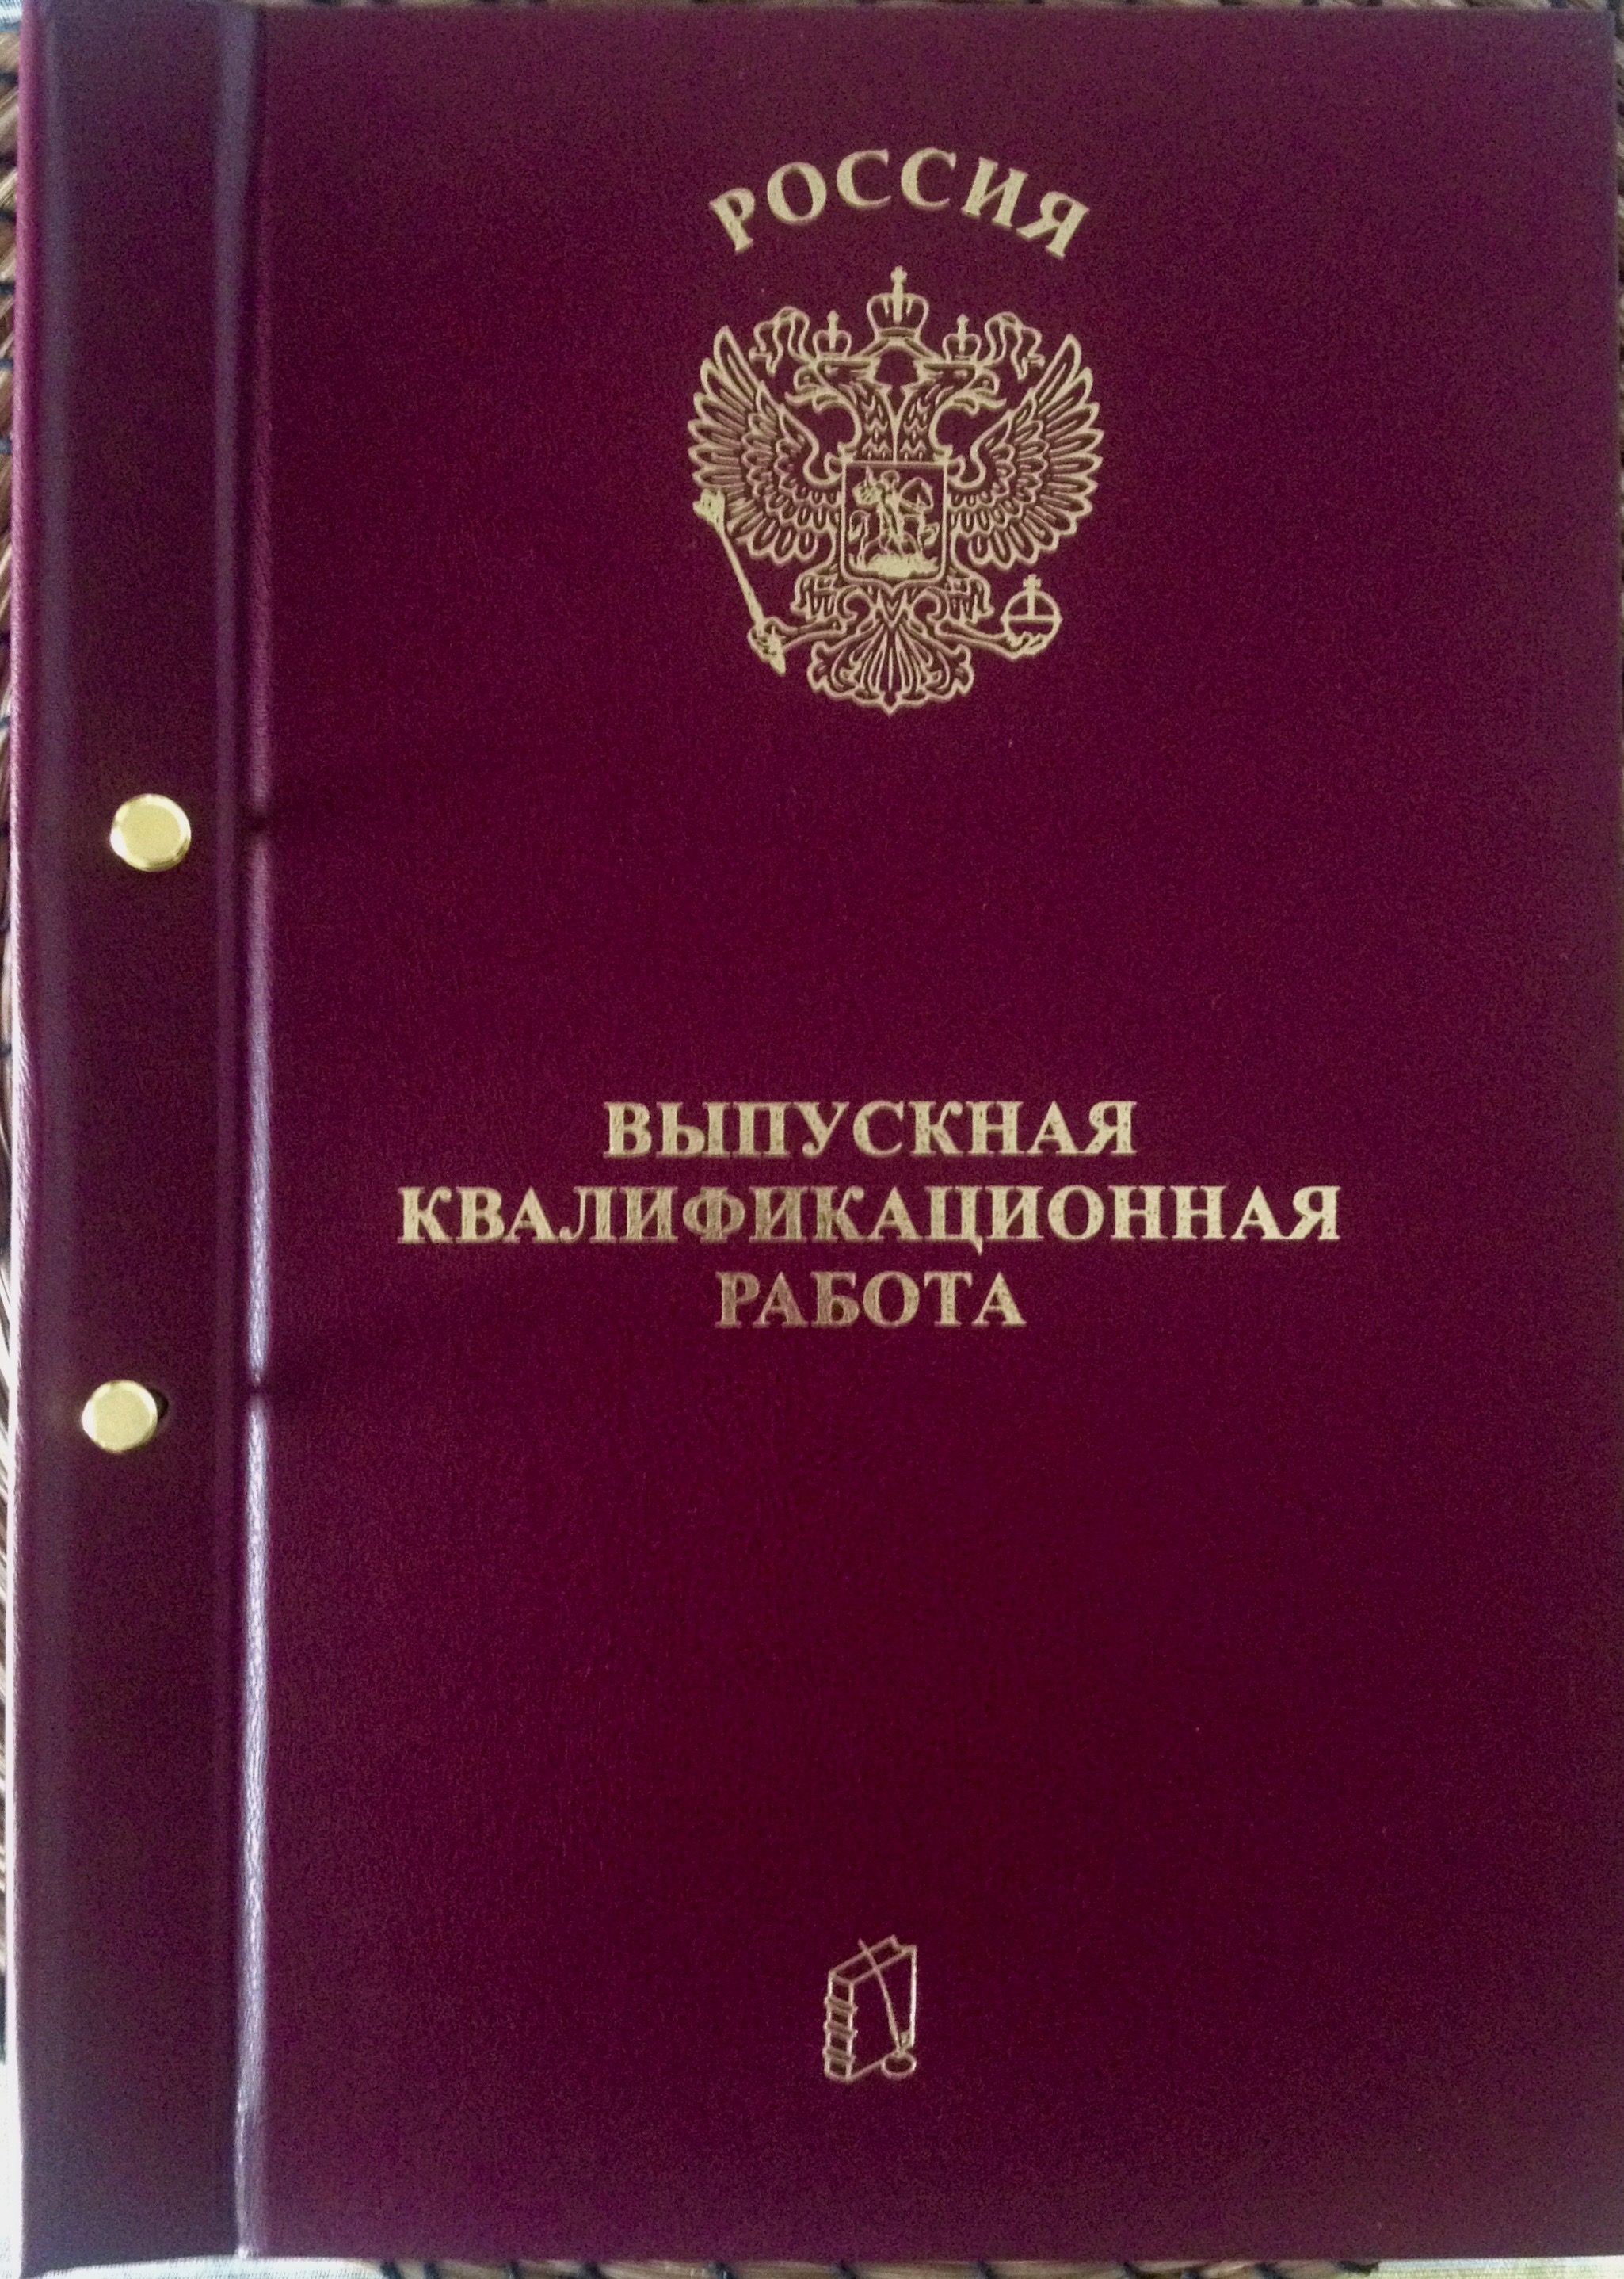
\includegraphics[height=3.5in]{figures/binding.jpeg}
    \vspace*{-4mm}
    \caption{Binding book for diploma work}
    \label{fig:binding}
\end{figure}